\documentclass[twoside]{book}

% Packages required by doxygen
\usepackage{fixltx2e}
\usepackage{calc}
\usepackage{doxygen}
\usepackage[export]{adjustbox} % also loads graphicx
\usepackage{graphicx}
\usepackage[utf8]{inputenc}
\usepackage{makeidx}
\usepackage{multicol}
\usepackage{multirow}
\PassOptionsToPackage{warn}{textcomp}
\usepackage{textcomp}
\usepackage[nointegrals]{wasysym}
\usepackage[table]{xcolor}

% Font selection
\usepackage[T1]{fontenc}
\usepackage[scaled=.90]{helvet}
\usepackage{courier}
\usepackage{amssymb}
\usepackage{sectsty}
\renewcommand{\familydefault}{\sfdefault}
\allsectionsfont{%
  \fontseries{bc}\selectfont%
  \color{darkgray}%
}
\renewcommand{\DoxyLabelFont}{%
  \fontseries{bc}\selectfont%
  \color{darkgray}%
}
\newcommand{\+}{\discretionary{\mbox{\scriptsize$\hookleftarrow$}}{}{}}

% Page & text layout
\usepackage{geometry}
\geometry{%
  a4paper,%
  top=2.5cm,%
  bottom=2.5cm,%
  left=2.5cm,%
  right=2.5cm%
}
\tolerance=750
\hfuzz=15pt
\hbadness=750
\setlength{\emergencystretch}{15pt}
\setlength{\parindent}{0cm}
\setlength{\parskip}{3ex plus 2ex minus 2ex}
\makeatletter
\renewcommand{\paragraph}{%
  \@startsection{paragraph}{4}{0ex}{-1.0ex}{1.0ex}{%
    \normalfont\normalsize\bfseries\SS@parafont%
  }%
}
\renewcommand{\subparagraph}{%
  \@startsection{subparagraph}{5}{0ex}{-1.0ex}{1.0ex}{%
    \normalfont\normalsize\bfseries\SS@subparafont%
  }%
}
\makeatother

% Headers & footers
\usepackage{fancyhdr}
\pagestyle{fancyplain}
\fancyhead[LE]{\fancyplain{}{\bfseries\thepage}}
\fancyhead[CE]{\fancyplain{}{}}
\fancyhead[RE]{\fancyplain{}{\bfseries\leftmark}}
\fancyhead[LO]{\fancyplain{}{\bfseries\rightmark}}
\fancyhead[CO]{\fancyplain{}{}}
\fancyhead[RO]{\fancyplain{}{\bfseries\thepage}}
\fancyfoot[LE]{\fancyplain{}{}}
\fancyfoot[CE]{\fancyplain{}{}}
\fancyfoot[RE]{\fancyplain{}{\bfseries\scriptsize Generated by Doxygen }}
\fancyfoot[LO]{\fancyplain{}{\bfseries\scriptsize Generated by Doxygen }}
\fancyfoot[CO]{\fancyplain{}{}}
\fancyfoot[RO]{\fancyplain{}{}}
\renewcommand{\footrulewidth}{0.4pt}
\renewcommand{\chaptermark}[1]{%
  \markboth{#1}{}%
}
\renewcommand{\sectionmark}[1]{%
  \markright{\thesection\ #1}%
}

% Indices & bibliography
\usepackage{natbib}
\usepackage[titles]{tocloft}
\setcounter{tocdepth}{3}
\setcounter{secnumdepth}{5}
\makeindex

% Hyperlinks (required, but should be loaded last)
\usepackage{ifpdf}
\ifpdf
  \usepackage[pdftex,pagebackref=true]{hyperref}
\else
  \usepackage[ps2pdf,pagebackref=true]{hyperref}
\fi
\hypersetup{%
  colorlinks=true,%
  linkcolor=blue,%
  citecolor=blue,%
  unicode%
}

% Custom commands
\newcommand{\clearemptydoublepage}{%
  \newpage{\pagestyle{empty}\cleardoublepage}%
}

\usepackage{caption}
\captionsetup{labelsep=space,justification=centering,font={bf},singlelinecheck=off,skip=4pt,position=top}

%===== C O N T E N T S =====

\begin{document}

% Titlepage & ToC
\hypersetup{pageanchor=false,
             bookmarksnumbered=true,
             pdfencoding=unicode
            }
\pagenumbering{alph}
\begin{titlepage}
\vspace*{7cm}
\begin{center}%
{\Large My Project }\\
\vspace*{1cm}
{\large Generated by Doxygen 1.8.13}\\
\end{center}
\end{titlepage}
\clearemptydoublepage
\pagenumbering{roman}
\tableofcontents
\clearemptydoublepage
\pagenumbering{arabic}
\hypersetup{pageanchor=true}

%--- Begin generated contents ---
\chapter{Data Structure Index}
\section{Data Structures}
Here are the data structures with brief descriptions\+:\begin{DoxyCompactList}
\item\contentsline{section}{\hyperlink{structentity}{entity} }{\pageref{structentity}}{}
\item\contentsline{section}{\hyperlink{structquiz}{quiz} }{\pageref{structquiz}}{}
\item\contentsline{section}{\hyperlink{structrest}{rest} }{\pageref{structrest}}{}
\end{DoxyCompactList}

\chapter{File Index}
\section{File List}
Here is a list of all files with brief descriptions\+:\begin{DoxyCompactList}
\item\contentsline{section}{\hyperlink{create_8c}{create.\+c} \\*Dans ce fichier deux fichiers binaires fait les appelles }{\pageref{create_8c}}{}
\item\contentsline{section}{\hyperlink{main_8c}{main.\+c} \\*Circuit enigme quiz }{\pageref{main_8c}}{}
\item\contentsline{section}{\hyperlink{quiz_8c}{quiz.\+c} \\*Il y a ici tous les fonctions de l\textquotesingle{}enigme quiz }{\pageref{quiz_8c}}{}
\item\contentsline{section}{\hyperlink{quiz_8h}{quiz.\+h} \\*Il y a ici les structures et la liaison des procedures de l\textquotesingle{}enigme }{\pageref{quiz_8h}}{}
\end{DoxyCompactList}

\chapter{Data Structure Documentation}
\hypertarget{structserrure}{}\section{serrure Struct Reference}
\label{structserrure}\index{serrure@{serrure}}


il y a ici les structures et la liaison des procedures de l\textquotesingle{}enigme.  




{\ttfamily \#include $<$enigme1.\+h$>$}

\subsection*{Data Fields}
\begin{DoxyCompactItemize}
\item 
S\+D\+L\+\_\+\+Surface $\ast$ \hyperlink{structserrure_a2bf4f397971a1bcebad46980e7bfedc0}{image}
\item 
S\+D\+L\+\_\+\+Rect \hyperlink{structserrure_a8cd1a53719ab1611f0332885c5a988d0}{pos}
\end{DoxyCompactItemize}


\subsection{Detailed Description}
il y a ici les structures et la liaison des procedures de l\textquotesingle{}enigme. 

\subsection{Field Documentation}
\mbox{\Hypertarget{structserrure_a2bf4f397971a1bcebad46980e7bfedc0}\label{structserrure_a2bf4f397971a1bcebad46980e7bfedc0}} 
\index{serrure@{serrure}!image@{image}}
\index{image@{image}!serrure@{serrure}}
\subsubsection{\texorpdfstring{image}{image}}
{\footnotesize\ttfamily S\+D\+L\+\_\+\+Surface $\ast$ serrure\+::image}

\mbox{\Hypertarget{structserrure_a8cd1a53719ab1611f0332885c5a988d0}\label{structserrure_a8cd1a53719ab1611f0332885c5a988d0}} 
\index{serrure@{serrure}!pos@{pos}}
\index{pos@{pos}!serrure@{serrure}}
\subsubsection{\texorpdfstring{pos}{pos}}
{\footnotesize\ttfamily S\+D\+L\+\_\+\+Rect serrure\+::pos}



The documentation for this struct was generated from the following files\+:\begin{DoxyCompactItemize}
\item 
\hyperlink{enigme1_8c}{enigme1.\+c}\item 
\hyperlink{enigme1_8h}{enigme1.\+h}\item 
\hyperlink{lock_8h}{lock.\+h}\end{DoxyCompactItemize}

\chapter{File Documentation}
\hypertarget{enigme1_8c}{}\section{enigme1.\+c File Reference}
\label{enigme1_8c}\index{enigme1.\+c@{enigme1.\+c}}
{\ttfamily \#include $<$stdio.\+h$>$}\newline
{\ttfamily \#include $<$stdlib.\+h$>$}\newline
{\ttfamily \#include $<$time.\+h$>$}\newline
{\ttfamily \#include \char`\"{}/usr/include/\+S\+D\+L/\+S\+D\+L.\+h\char`\"{}}\newline
{\ttfamily \#include \char`\"{}/usr/include/\+S\+D\+L/\+S\+D\+L\+\_\+image.\+h\char`\"{}}\newline
{\ttfamily \#include \char`\"{}/usr/include/\+S\+D\+L/\+S\+D\+L\+\_\+mixer.\+h\char`\"{}}\newline
{\ttfamily \#include \char`\"{}/usr/include/\+S\+D\+L/\+S\+D\+L\+\_\+rotozoom.\+h\char`\"{}}\newline
Include dependency graph for enigme1.\+c\+:\nopagebreak
\begin{figure}[H]
\begin{center}
\leavevmode

\includegraphics[width=350pt]{enigme1_8c__incl}
\end{center}
\end{figure}
\subsection*{Data Structures}
\begin{DoxyCompactItemize}
\item 
struct \hyperlink{structserrure}{serrure}
\begin{DoxyCompactList}\small\item\em il y a ici les structures et la liaison des procedures de l\textquotesingle{}enigme. \end{DoxyCompactList}\end{DoxyCompactItemize}
\subsection*{Functions}
\begin{DoxyCompactItemize}
\item 
int \hyperlink{enigme1_8c_a8f387384696c4294f1521ad662b556db}{hover} (S\+D\+L\+\_\+\+Rect pos, int x, int y)
\item 
void \hyperlink{enigme1_8c_acdef7a1fd863a6d3770c1268cb06add3}{main} ()
\end{DoxyCompactItemize}


\subsection{Function Documentation}
\mbox{\Hypertarget{enigme1_8c_a8f387384696c4294f1521ad662b556db}\label{enigme1_8c_a8f387384696c4294f1521ad662b556db}} 
\index{enigme1.\+c@{enigme1.\+c}!hover@{hover}}
\index{hover@{hover}!enigme1.\+c@{enigme1.\+c}}
\subsubsection{\texorpdfstring{hover()}{hover()}}
{\footnotesize\ttfamily int hover (\begin{DoxyParamCaption}\item[{S\+D\+L\+\_\+\+Rect}]{pos,  }\item[{int}]{x,  }\item[{int}]{y }\end{DoxyParamCaption})}

Here is the caller graph for this function\+:
\nopagebreak
\begin{figure}[H]
\begin{center}
\leavevmode
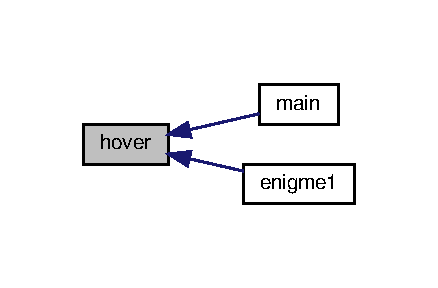
\includegraphics[width=210pt]{enigme1_8c_a8f387384696c4294f1521ad662b556db_icgraph}
\end{center}
\end{figure}
\mbox{\Hypertarget{enigme1_8c_acdef7a1fd863a6d3770c1268cb06add3}\label{enigme1_8c_acdef7a1fd863a6d3770c1268cb06add3}} 
\index{enigme1.\+c@{enigme1.\+c}!main@{main}}
\index{main@{main}!enigme1.\+c@{enigme1.\+c}}
\subsubsection{\texorpdfstring{main()}{main()}}
{\footnotesize\ttfamily void main (\begin{DoxyParamCaption}{ }\end{DoxyParamCaption})}

Here is the call graph for this function\+:
\nopagebreak
\begin{figure}[H]
\begin{center}
\leavevmode
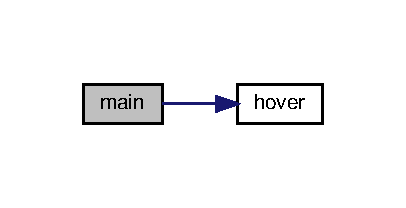
\includegraphics[width=195pt]{enigme1_8c_acdef7a1fd863a6d3770c1268cb06add3_cgraph}
\end{center}
\end{figure}

\hypertarget{enigme1_8h}{}\section{enigme1.\+h File Reference}
\label{enigme1_8h}\index{enigme1.\+h@{enigme1.\+h}}
\subsection*{Data Structures}
\begin{DoxyCompactItemize}
\item 
struct \hyperlink{structserrure}{serrure}
\begin{DoxyCompactList}\small\item\em il y a ici les structures et la liaison des procedures de l\textquotesingle{}enigme. \end{DoxyCompactList}\end{DoxyCompactItemize}
\subsection*{Functions}
\begin{DoxyCompactItemize}
\item 
void \hyperlink{enigme1_8h_a414b153524d43e221309cf892be790cf}{enigme1} (S\+D\+L\+\_\+\+Surface $\ast$screen, S\+D\+L\+\_\+\+Event event)
\end{DoxyCompactItemize}


\subsection{Function Documentation}
\mbox{\Hypertarget{enigme1_8h_a414b153524d43e221309cf892be790cf}\label{enigme1_8h_a414b153524d43e221309cf892be790cf}} 
\index{enigme1.\+h@{enigme1.\+h}!enigme1@{enigme1}}
\index{enigme1@{enigme1}!enigme1.\+h@{enigme1.\+h}}
\subsubsection{\texorpdfstring{enigme1()}{enigme1()}}
{\footnotesize\ttfamily void enigme1 (\begin{DoxyParamCaption}\item[{S\+D\+L\+\_\+\+Surface $\ast$}]{screen,  }\item[{S\+D\+L\+\_\+\+Event}]{event }\end{DoxyParamCaption})}

Here is the call graph for this function\+:\nopagebreak
\begin{figure}[H]
\begin{center}
\leavevmode
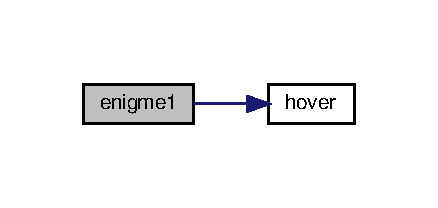
\includegraphics[width=210pt]{enigme1_8h_a414b153524d43e221309cf892be790cf_cgraph}
\end{center}
\end{figure}

\hypertarget{lock_8c}{}\section{lock.\+c File Reference}
\label{lock_8c}\index{lock.\+c@{lock.\+c}}


il y a ici tous les fonctions de l\textquotesingle{}enigme.  


{\ttfamily \#include $<$stdio.\+h$>$}\newline
{\ttfamily \#include $<$stdlib.\+h$>$}\newline
{\ttfamily \#include $<$time.\+h$>$}\newline
{\ttfamily \#include \char`\"{}/usr/include/\+S\+D\+L/\+S\+D\+L.\+h\char`\"{}}\newline
{\ttfamily \#include \char`\"{}/usr/include/\+S\+D\+L/\+S\+D\+L\+\_\+image.\+h\char`\"{}}\newline
{\ttfamily \#include \char`\"{}/usr/include/\+S\+D\+L/\+S\+D\+L\+\_\+mixer.\+h\char`\"{}}\newline
{\ttfamily \#include \char`\"{}/usr/include/\+S\+D\+L/\+S\+D\+L\+\_\+events.\+h\char`\"{}}\newline
{\ttfamily \#include \char`\"{}/usr/include/\+S\+D\+L/\+S\+D\+L\+\_\+mouse.\+h\char`\"{}}\newline
{\ttfamily \#include \char`\"{}/usr/include/\+S\+D\+L/\+S\+D\+L\+\_\+rotozoom.\+h\char`\"{}}\newline
{\ttfamily \#include \char`\"{}lock.\+h\char`\"{}}\newline
Include dependency graph for lock.\+c\+:\nopagebreak
\begin{figure}[H]
\begin{center}
\leavevmode
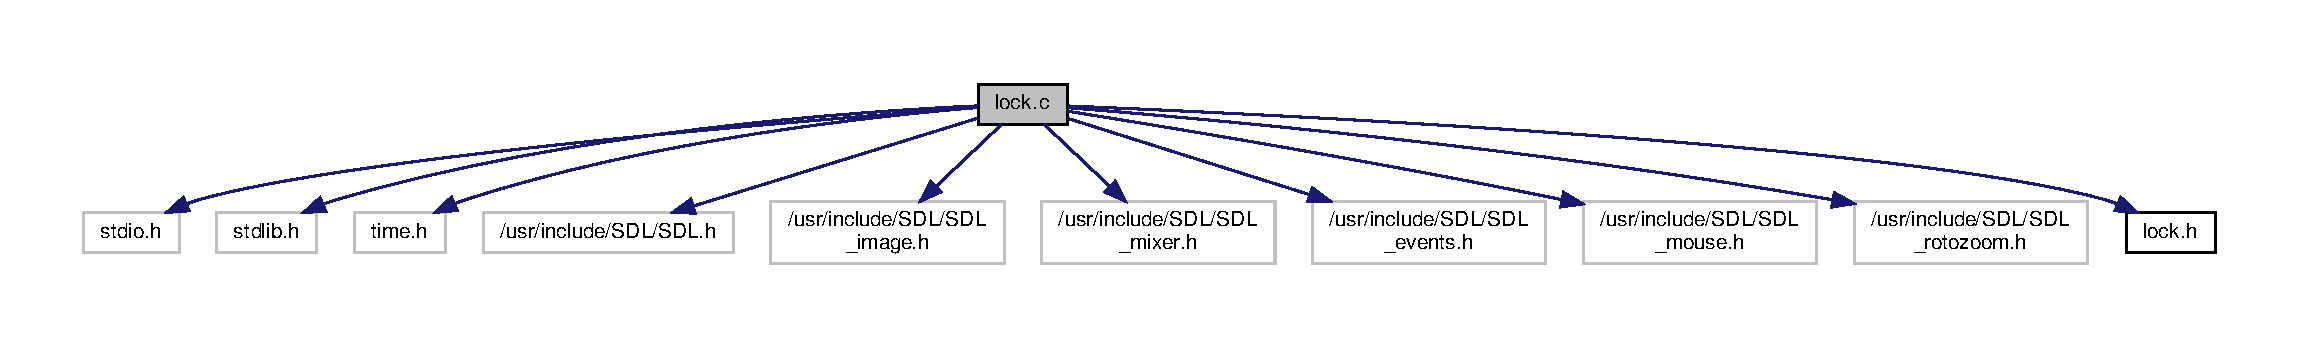
\includegraphics[width=350pt]{lock_8c__incl}
\end{center}
\end{figure}
\subsection*{Functions}
\begin{DoxyCompactItemize}
\item 
int \hyperlink{lock_8c_a8f387384696c4294f1521ad662b556db}{hover} (S\+D\+L\+\_\+\+Rect pos, int x, int y)
\item 
void \hyperlink{lock_8c_abd9d77bdfe0481d8d4475dac1b18fb12}{initialiser} (\hyperlink{structserrure}{serrure} $\ast$lock, \hyperlink{structserrure}{serrure} $\ast$lockpick, S\+D\+L\+\_\+\+Rect $\ast$rec, S\+D\+L\+\_\+\+Surface $\ast$$\ast$yaru)
\begin{DoxyCompactList}\small\item\em initialiser les donnees de l\textquotesingle{}enigme. \end{DoxyCompactList}\item 
void \hyperlink{lock_8c_a3dd80cb222a9d8b62d18dc6a84b21d06}{afficher} (int $\ast$vie, int $\ast$access, S\+D\+L\+\_\+\+Surface $\ast$screen, S\+D\+L\+\_\+\+Event event, \hyperlink{structserrure}{serrure} lock, \hyperlink{structserrure}{serrure} lockpick, S\+D\+L\+\_\+\+Rect $\ast$rec, S\+D\+L\+\_\+\+Surface $\ast$$\ast$yaru)
\begin{DoxyCompactList}\small\item\em afficher et modifier les donnees de l\textquotesingle{}enigme. \end{DoxyCompactList}\end{DoxyCompactItemize}


\subsection{Detailed Description}
il y a ici tous les fonctions de l\textquotesingle{}enigme. 



\subsection{Function Documentation}
\mbox{\Hypertarget{lock_8c_a3dd80cb222a9d8b62d18dc6a84b21d06}\label{lock_8c_a3dd80cb222a9d8b62d18dc6a84b21d06}} 
\index{lock.\+c@{lock.\+c}!afficher@{afficher}}
\index{afficher@{afficher}!lock.\+c@{lock.\+c}}
\subsubsection{\texorpdfstring{afficher()}{afficher()}}
{\footnotesize\ttfamily void afficher (\begin{DoxyParamCaption}\item[{int $\ast$}]{vie,  }\item[{int $\ast$}]{access,  }\item[{S\+D\+L\+\_\+\+Surface $\ast$}]{screen,  }\item[{S\+D\+L\+\_\+\+Event}]{event,  }\item[{\hyperlink{structserrure}{serrure}}]{lock,  }\item[{\hyperlink{structserrure}{serrure}}]{lockpick,  }\item[{S\+D\+L\+\_\+\+Rect $\ast$}]{rec,  }\item[{S\+D\+L\+\_\+\+Surface $\ast$$\ast$}]{yaru }\end{DoxyParamCaption})}



afficher et modifier les donnees de l\textquotesingle{}enigme. 


\begin{DoxyParams}{Parameters}
{\em int} & $\ast$vie \+: modifier vie si le personnage a cliquer dehors la serrure. \\
\hline
{\em int} & $\ast$access \+: modifie access si le personnage a completer l\textquotesingle{}enigme. \\
\hline
{\em S\+D\+L\+\_\+\+Surface$\ast$} & screen\+: afficher l\textquotesingle{}ecran. \\
\hline
{\em S\+D\+L\+\_\+\+Event} & event \+: fait les actions generer pas le hardware. \\
\hline
\end{DoxyParams}
\begin{DoxyReturn}{Returns}
Nothing 
\end{DoxyReturn}
Here is the call graph for this function\+:\nopagebreak
\begin{figure}[H]
\begin{center}
\leavevmode
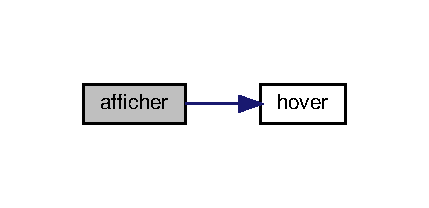
\includegraphics[width=206pt]{lock_8c_a3dd80cb222a9d8b62d18dc6a84b21d06_cgraph}
\end{center}
\end{figure}
Here is the caller graph for this function\+:\nopagebreak
\begin{figure}[H]
\begin{center}
\leavevmode
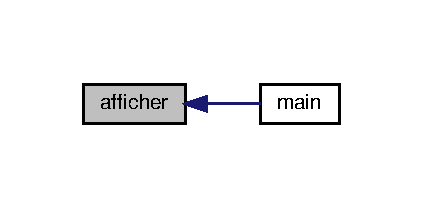
\includegraphics[width=203pt]{lock_8c_a3dd80cb222a9d8b62d18dc6a84b21d06_icgraph}
\end{center}
\end{figure}
\mbox{\Hypertarget{lock_8c_a8f387384696c4294f1521ad662b556db}\label{lock_8c_a8f387384696c4294f1521ad662b556db}} 
\index{lock.\+c@{lock.\+c}!hover@{hover}}
\index{hover@{hover}!lock.\+c@{lock.\+c}}
\subsubsection{\texorpdfstring{hover()}{hover()}}
{\footnotesize\ttfamily int hover (\begin{DoxyParamCaption}\item[{S\+D\+L\+\_\+\+Rect}]{pos,  }\item[{int}]{x,  }\item[{int}]{y }\end{DoxyParamCaption})}

Here is the caller graph for this function\+:\nopagebreak
\begin{figure}[H]
\begin{center}
\leavevmode
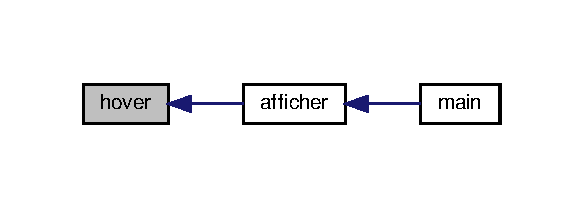
\includegraphics[width=280pt]{lock_8c_a8f387384696c4294f1521ad662b556db_icgraph}
\end{center}
\end{figure}
\mbox{\Hypertarget{lock_8c_abd9d77bdfe0481d8d4475dac1b18fb12}\label{lock_8c_abd9d77bdfe0481d8d4475dac1b18fb12}} 
\index{lock.\+c@{lock.\+c}!initialiser@{initialiser}}
\index{initialiser@{initialiser}!lock.\+c@{lock.\+c}}
\subsubsection{\texorpdfstring{initialiser()}{initialiser()}}
{\footnotesize\ttfamily void initialiser (\begin{DoxyParamCaption}\item[{\hyperlink{structserrure}{serrure} $\ast$}]{lock,  }\item[{\hyperlink{structserrure}{serrure} $\ast$}]{lockpick,  }\item[{S\+D\+L\+\_\+\+Rect $\ast$}]{rec,  }\item[{S\+D\+L\+\_\+\+Surface $\ast$$\ast$}]{yaru }\end{DoxyParamCaption})}



initialiser les donnees de l\textquotesingle{}enigme. 


\begin{DoxyParams}{Parameters}
{\em serrure} & $\ast$lock \+: adresse pour changer avec surface et position du serrure. \\
\hline
{\em serrure} & $\ast$lockprick \+: adresse pour changer avec surface et position du poignée. \\
\hline
{\em S\+D\+L\+\_\+\+Rect} & $\ast$rec \+: adresse pour changer la position du rotozoom du serrure. \\
\hline
{\em S\+D\+L\+\_\+\+Rect$\ast$} & $\ast$yaru \+: adresse pour changer la taille et l\textquotesingle{}angle du serrure. \\
\hline
\end{DoxyParams}
\begin{DoxyReturn}{Returns}
Initialisation de l\textquotesingle{}enigme 
\end{DoxyReturn}
Here is the caller graph for this function\+:\nopagebreak
\begin{figure}[H]
\begin{center}
\leavevmode
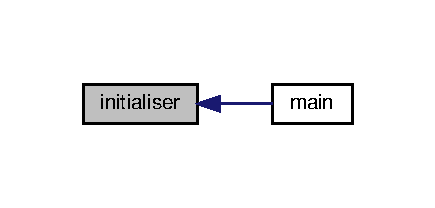
\includegraphics[width=209pt]{lock_8c_abd9d77bdfe0481d8d4475dac1b18fb12_icgraph}
\end{center}
\end{figure}

\hypertarget{lock_8h}{}\section{lock.\+h File Reference}
\label{lock_8h}\index{lock.\+h@{lock.\+h}}
This graph shows which files directly or indirectly include this file\+:
\nopagebreak
\begin{figure}[H]
\begin{center}
\leavevmode
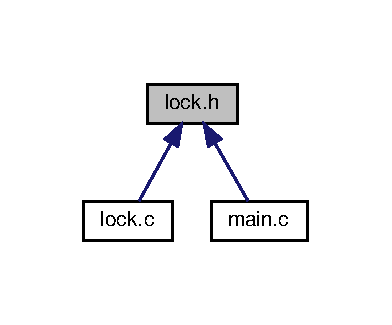
\includegraphics[width=188pt]{lock_8h__dep__incl}
\end{center}
\end{figure}
\subsection*{Data Structures}
\begin{DoxyCompactItemize}
\item 
struct \hyperlink{structserrure}{serrure}
\begin{DoxyCompactList}\small\item\em il y a ici les structures et la liaison des procedures de l\textquotesingle{}enigme. \end{DoxyCompactList}\end{DoxyCompactItemize}
\subsection*{Functions}
\begin{DoxyCompactItemize}
\item 
void \hyperlink{lock_8h_abd9d77bdfe0481d8d4475dac1b18fb12}{initialiser} (\hyperlink{structserrure}{serrure} $\ast$lock, \hyperlink{structserrure}{serrure} $\ast$lockpick, S\+D\+L\+\_\+\+Rect $\ast$rec, S\+D\+L\+\_\+\+Surface $\ast$$\ast$yaru)
\begin{DoxyCompactList}\small\item\em initialiser les donnees de l\textquotesingle{}enigme. \end{DoxyCompactList}\item 
void \hyperlink{lock_8h_a3dd80cb222a9d8b62d18dc6a84b21d06}{afficher} (int $\ast$vie, int $\ast$access, S\+D\+L\+\_\+\+Surface $\ast$screen, S\+D\+L\+\_\+\+Event event, \hyperlink{structserrure}{serrure} lock, \hyperlink{structserrure}{serrure} lockpick, S\+D\+L\+\_\+\+Rect $\ast$rec, S\+D\+L\+\_\+\+Surface $\ast$$\ast$yaru)
\begin{DoxyCompactList}\small\item\em afficher et modifier les donnees de l\textquotesingle{}enigme. \end{DoxyCompactList}\end{DoxyCompactItemize}


\subsection{Function Documentation}
\mbox{\Hypertarget{lock_8h_a3dd80cb222a9d8b62d18dc6a84b21d06}\label{lock_8h_a3dd80cb222a9d8b62d18dc6a84b21d06}} 
\index{lock.\+h@{lock.\+h}!afficher@{afficher}}
\index{afficher@{afficher}!lock.\+h@{lock.\+h}}
\subsubsection{\texorpdfstring{afficher()}{afficher()}}
{\footnotesize\ttfamily void afficher (\begin{DoxyParamCaption}\item[{int $\ast$}]{vie,  }\item[{int $\ast$}]{access,  }\item[{S\+D\+L\+\_\+\+Surface $\ast$}]{screen,  }\item[{S\+D\+L\+\_\+\+Event}]{event,  }\item[{\hyperlink{structserrure}{serrure}}]{lock,  }\item[{\hyperlink{structserrure}{serrure}}]{lockpick,  }\item[{S\+D\+L\+\_\+\+Rect $\ast$}]{rec,  }\item[{S\+D\+L\+\_\+\+Surface $\ast$$\ast$}]{yaru }\end{DoxyParamCaption})}



afficher et modifier les donnees de l\textquotesingle{}enigme. 


\begin{DoxyParams}{Parameters}
{\em int} & $\ast$vie \+: modifier vie si le personnage a cliquer dehors la serrure. \\
\hline
{\em int} & $\ast$access \+: modifie access si le personnage a completer l\textquotesingle{}enigme. \\
\hline
{\em S\+D\+L\+\_\+\+Surface$\ast$} & screen\+: afficher l\textquotesingle{}ecran. \\
\hline
{\em S\+D\+L\+\_\+\+Event} & event \+: fait les actions generer pas le hardware. \\
\hline
\end{DoxyParams}
\begin{DoxyReturn}{Returns}
Nothing 
\end{DoxyReturn}
Here is the call graph for this function\+:\nopagebreak
\begin{figure}[H]
\begin{center}
\leavevmode
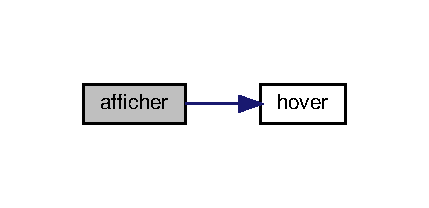
\includegraphics[width=206pt]{lock_8h_a3dd80cb222a9d8b62d18dc6a84b21d06_cgraph}
\end{center}
\end{figure}
Here is the caller graph for this function\+:\nopagebreak
\begin{figure}[H]
\begin{center}
\leavevmode
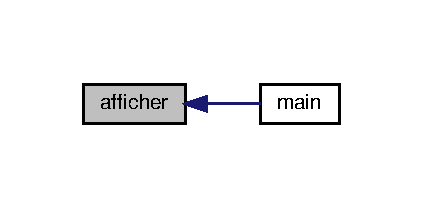
\includegraphics[width=203pt]{lock_8h_a3dd80cb222a9d8b62d18dc6a84b21d06_icgraph}
\end{center}
\end{figure}
\mbox{\Hypertarget{lock_8h_abd9d77bdfe0481d8d4475dac1b18fb12}\label{lock_8h_abd9d77bdfe0481d8d4475dac1b18fb12}} 
\index{lock.\+h@{lock.\+h}!initialiser@{initialiser}}
\index{initialiser@{initialiser}!lock.\+h@{lock.\+h}}
\subsubsection{\texorpdfstring{initialiser()}{initialiser()}}
{\footnotesize\ttfamily void initialiser (\begin{DoxyParamCaption}\item[{\hyperlink{structserrure}{serrure} $\ast$}]{lock,  }\item[{\hyperlink{structserrure}{serrure} $\ast$}]{lockpick,  }\item[{S\+D\+L\+\_\+\+Rect $\ast$}]{rec,  }\item[{S\+D\+L\+\_\+\+Surface $\ast$$\ast$}]{yaru }\end{DoxyParamCaption})}



initialiser les donnees de l\textquotesingle{}enigme. 


\begin{DoxyParams}{Parameters}
{\em serrure} & $\ast$lock \+: adresse pour changer avec surface et position du serrure. \\
\hline
{\em serrure} & $\ast$lockprick \+: adresse pour changer avec surface et position du poignée. \\
\hline
{\em S\+D\+L\+\_\+\+Rect} & $\ast$rec \+: adresse pour changer la position du rotozoom du serrure. \\
\hline
{\em S\+D\+L\+\_\+\+Rect$\ast$} & $\ast$yaru \+: adresse pour changer la taille et l\textquotesingle{}angle du serrure. \\
\hline
\end{DoxyParams}
\begin{DoxyReturn}{Returns}
Initialisation de l\textquotesingle{}enigme 
\end{DoxyReturn}
Here is the caller graph for this function\+:\nopagebreak
\begin{figure}[H]
\begin{center}
\leavevmode
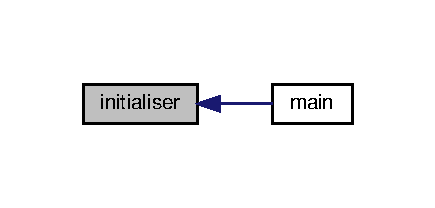
\includegraphics[width=209pt]{lock_8h_abd9d77bdfe0481d8d4475dac1b18fb12_icgraph}
\end{center}
\end{figure}

\hypertarget{main_8c}{}\section{main.\+c File Reference}
\label{main_8c}\index{main.\+c@{main.\+c}}


circuit enigme.  


{\ttfamily \#include $<$stdio.\+h$>$}\newline
{\ttfamily \#include $<$stdlib.\+h$>$}\newline
{\ttfamily \#include $<$time.\+h$>$}\newline
{\ttfamily \#include \char`\"{}/usr/include/\+S\+D\+L/\+S\+D\+L.\+h\char`\"{}}\newline
{\ttfamily \#include \char`\"{}/usr/include/\+S\+D\+L/\+S\+D\+L\+\_\+image.\+h\char`\"{}}\newline
{\ttfamily \#include \char`\"{}/usr/include/\+S\+D\+L/\+S\+D\+L\+\_\+mixer.\+h\char`\"{}}\newline
{\ttfamily \#include \char`\"{}/usr/include/\+S\+D\+L/\+S\+D\+L\+\_\+events.\+h\char`\"{}}\newline
{\ttfamily \#include \char`\"{}/usr/include/\+S\+D\+L/\+S\+D\+L\+\_\+mouse.\+h\char`\"{}}\newline
{\ttfamily \#include \char`\"{}circuit.\+h\char`\"{}}\newline
Include dependency graph for main.\+c\+:
\nopagebreak
\begin{figure}[H]
\begin{center}
\leavevmode
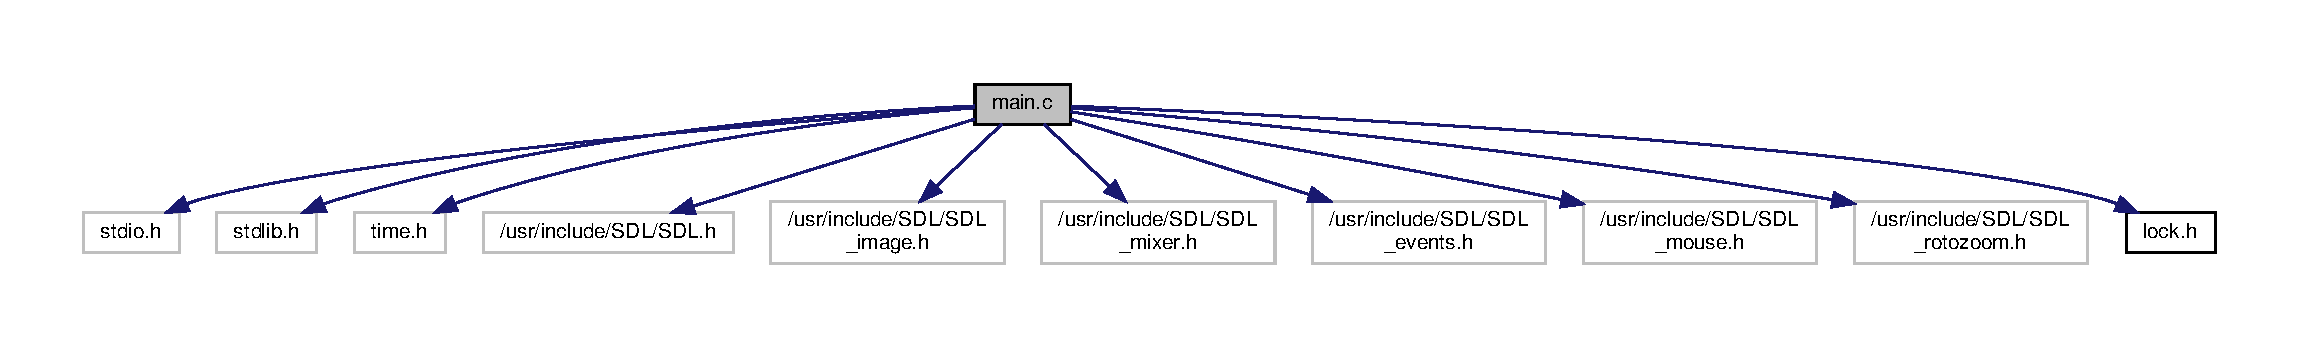
\includegraphics[width=350pt]{main_8c__incl}
\end{center}
\end{figure}
\subsection*{Functions}
\begin{DoxyCompactItemize}
\item 
int \hyperlink{main_8c_ae66f6b31b5ad750f1fe042a706a4e3d4}{main} ()
\end{DoxyCompactItemize}


\subsection{Detailed Description}
circuit enigme. 

\begin{DoxyAuthor}{Author}
Blindspot 
\end{DoxyAuthor}
\begin{DoxyVersion}{Version}
0.\+1 
\end{DoxyVersion}
\begin{DoxyDate}{Date}
M\+AY 06, 2019 
\end{DoxyDate}


\subsection{Function Documentation}
\mbox{\Hypertarget{main_8c_ae66f6b31b5ad750f1fe042a706a4e3d4}\label{main_8c_ae66f6b31b5ad750f1fe042a706a4e3d4}} 
\index{main.\+c@{main.\+c}!main@{main}}
\index{main@{main}!main.\+c@{main.\+c}}
\subsubsection{\texorpdfstring{main()}{main()}}
{\footnotesize\ttfamily int main (\begin{DoxyParamCaption}{ }\end{DoxyParamCaption})}

Here is the call graph for this function\+:\nopagebreak
\begin{figure}[H]
\begin{center}
\leavevmode
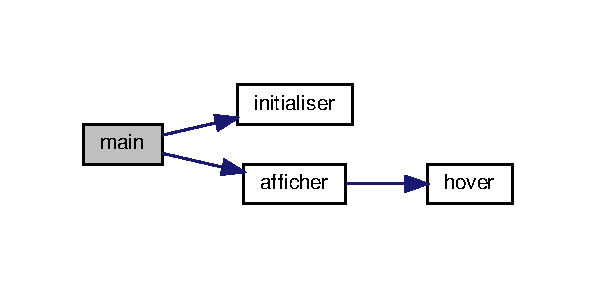
\includegraphics[width=286pt]{main_8c_ae66f6b31b5ad750f1fe042a706a4e3d4_cgraph}
\end{center}
\end{figure}

\hypertarget{procedure_8c}{}\section{procedure.\+c File Reference}
\label{procedure_8c}\index{procedure.\+c@{procedure.\+c}}
\subsection*{Functions}
\begin{DoxyCompactItemize}
\item 
void \hyperlink{procedure_8c_a414b153524d43e221309cf892be790cf}{enigme1} (S\+D\+L\+\_\+\+Surface $\ast$screen, S\+D\+L\+\_\+\+Event event)
\end{DoxyCompactItemize}


\subsection{Function Documentation}
\mbox{\Hypertarget{procedure_8c_a414b153524d43e221309cf892be790cf}\label{procedure_8c_a414b153524d43e221309cf892be790cf}} 
\index{procedure.\+c@{procedure.\+c}!enigme1@{enigme1}}
\index{enigme1@{enigme1}!procedure.\+c@{procedure.\+c}}
\subsubsection{\texorpdfstring{enigme1()}{enigme1()}}
{\footnotesize\ttfamily void enigme1 (\begin{DoxyParamCaption}\item[{S\+D\+L\+\_\+\+Surface $\ast$}]{screen,  }\item[{S\+D\+L\+\_\+\+Event}]{event }\end{DoxyParamCaption})}

Here is the call graph for this function\+:\nopagebreak
\begin{figure}[H]
\begin{center}
\leavevmode
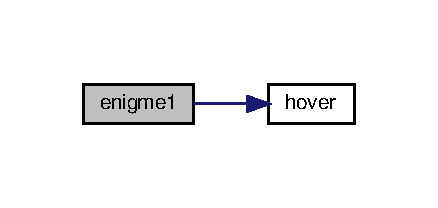
\includegraphics[width=210pt]{procedure_8c_a414b153524d43e221309cf892be790cf_cgraph}
\end{center}
\end{figure}

%--- End generated contents ---

% Index
\backmatter
\newpage
\phantomsection
\clearemptydoublepage
\addcontentsline{toc}{chapter}{Index}
\printindex

\end{document}
